% Options for packages loaded elsewhere
\PassOptionsToPackage{unicode}{hyperref}
\PassOptionsToPackage{hyphens}{url}
%
\documentclass[
]{article}
\usepackage{amsmath,amssymb}
\usepackage{lmodern}
\usepackage{iftex}
\ifPDFTeX
  \usepackage[T1]{fontenc}
  \usepackage[utf8]{inputenc}
  \usepackage{textcomp} % provide euro and other symbols
\else % if luatex or xetex
  \usepackage{unicode-math}
  \defaultfontfeatures{Scale=MatchLowercase}
  \defaultfontfeatures[\rmfamily]{Ligatures=TeX,Scale=1}
\fi
% Use upquote if available, for straight quotes in verbatim environments
\IfFileExists{upquote.sty}{\usepackage{upquote}}{}
\IfFileExists{microtype.sty}{% use microtype if available
  \usepackage[]{microtype}
  \UseMicrotypeSet[protrusion]{basicmath} % disable protrusion for tt fonts
}{}
\makeatletter
\@ifundefined{KOMAClassName}{% if non-KOMA class
  \IfFileExists{parskip.sty}{%
    \usepackage{parskip}
  }{% else
    \setlength{\parindent}{0pt}
    \setlength{\parskip}{6pt plus 2pt minus 1pt}}
}{% if KOMA class
  \KOMAoptions{parskip=half}}
\makeatother
\usepackage{xcolor}
\usepackage[margin=1in]{geometry}
\usepackage{color}
\usepackage{fancyvrb}
\newcommand{\VerbBar}{|}
\newcommand{\VERB}{\Verb[commandchars=\\\{\}]}
\DefineVerbatimEnvironment{Highlighting}{Verbatim}{commandchars=\\\{\}}
% Add ',fontsize=\small' for more characters per line
\usepackage{framed}
\definecolor{shadecolor}{RGB}{248,248,248}
\newenvironment{Shaded}{\begin{snugshade}}{\end{snugshade}}
\newcommand{\AlertTok}[1]{\textcolor[rgb]{0.94,0.16,0.16}{#1}}
\newcommand{\AnnotationTok}[1]{\textcolor[rgb]{0.56,0.35,0.01}{\textbf{\textit{#1}}}}
\newcommand{\AttributeTok}[1]{\textcolor[rgb]{0.77,0.63,0.00}{#1}}
\newcommand{\BaseNTok}[1]{\textcolor[rgb]{0.00,0.00,0.81}{#1}}
\newcommand{\BuiltInTok}[1]{#1}
\newcommand{\CharTok}[1]{\textcolor[rgb]{0.31,0.60,0.02}{#1}}
\newcommand{\CommentTok}[1]{\textcolor[rgb]{0.56,0.35,0.01}{\textit{#1}}}
\newcommand{\CommentVarTok}[1]{\textcolor[rgb]{0.56,0.35,0.01}{\textbf{\textit{#1}}}}
\newcommand{\ConstantTok}[1]{\textcolor[rgb]{0.00,0.00,0.00}{#1}}
\newcommand{\ControlFlowTok}[1]{\textcolor[rgb]{0.13,0.29,0.53}{\textbf{#1}}}
\newcommand{\DataTypeTok}[1]{\textcolor[rgb]{0.13,0.29,0.53}{#1}}
\newcommand{\DecValTok}[1]{\textcolor[rgb]{0.00,0.00,0.81}{#1}}
\newcommand{\DocumentationTok}[1]{\textcolor[rgb]{0.56,0.35,0.01}{\textbf{\textit{#1}}}}
\newcommand{\ErrorTok}[1]{\textcolor[rgb]{0.64,0.00,0.00}{\textbf{#1}}}
\newcommand{\ExtensionTok}[1]{#1}
\newcommand{\FloatTok}[1]{\textcolor[rgb]{0.00,0.00,0.81}{#1}}
\newcommand{\FunctionTok}[1]{\textcolor[rgb]{0.00,0.00,0.00}{#1}}
\newcommand{\ImportTok}[1]{#1}
\newcommand{\InformationTok}[1]{\textcolor[rgb]{0.56,0.35,0.01}{\textbf{\textit{#1}}}}
\newcommand{\KeywordTok}[1]{\textcolor[rgb]{0.13,0.29,0.53}{\textbf{#1}}}
\newcommand{\NormalTok}[1]{#1}
\newcommand{\OperatorTok}[1]{\textcolor[rgb]{0.81,0.36,0.00}{\textbf{#1}}}
\newcommand{\OtherTok}[1]{\textcolor[rgb]{0.56,0.35,0.01}{#1}}
\newcommand{\PreprocessorTok}[1]{\textcolor[rgb]{0.56,0.35,0.01}{\textit{#1}}}
\newcommand{\RegionMarkerTok}[1]{#1}
\newcommand{\SpecialCharTok}[1]{\textcolor[rgb]{0.00,0.00,0.00}{#1}}
\newcommand{\SpecialStringTok}[1]{\textcolor[rgb]{0.31,0.60,0.02}{#1}}
\newcommand{\StringTok}[1]{\textcolor[rgb]{0.31,0.60,0.02}{#1}}
\newcommand{\VariableTok}[1]{\textcolor[rgb]{0.00,0.00,0.00}{#1}}
\newcommand{\VerbatimStringTok}[1]{\textcolor[rgb]{0.31,0.60,0.02}{#1}}
\newcommand{\WarningTok}[1]{\textcolor[rgb]{0.56,0.35,0.01}{\textbf{\textit{#1}}}}
\usepackage{graphicx}
\makeatletter
\def\maxwidth{\ifdim\Gin@nat@width>\linewidth\linewidth\else\Gin@nat@width\fi}
\def\maxheight{\ifdim\Gin@nat@height>\textheight\textheight\else\Gin@nat@height\fi}
\makeatother
% Scale images if necessary, so that they will not overflow the page
% margins by default, and it is still possible to overwrite the defaults
% using explicit options in \includegraphics[width, height, ...]{}
\setkeys{Gin}{width=\maxwidth,height=\maxheight,keepaspectratio}
% Set default figure placement to htbp
\makeatletter
\def\fps@figure{htbp}
\makeatother
\setlength{\emergencystretch}{3em} % prevent overfull lines
\providecommand{\tightlist}{%
  \setlength{\itemsep}{0pt}\setlength{\parskip}{0pt}}
\setcounter{secnumdepth}{5}
\ifLuaTeX
  \usepackage{selnolig}  % disable illegal ligatures
\fi
\IfFileExists{bookmark.sty}{\usepackage{bookmark}}{\usepackage{hyperref}}
\IfFileExists{xurl.sty}{\usepackage{xurl}}{} % add URL line breaks if available
\urlstyle{same} % disable monospaced font for URLs
\hypersetup{
  pdftitle={Taller 2 Regresión lineal Multiple},
  pdfauthor={Andrés Felipe Palomino - David Stiven Rojas},
  hidelinks,
  pdfcreator={LaTeX via pandoc}}

\title{Taller 2 Regresión lineal Multiple}
\author{Andrés Felipe Palomino - David Stiven Rojas}
\date{2023-04-21}

\begin{document}
\maketitle

\hypertarget{introducciuxf3n}{%
\section{Introducción}\label{introducciuxf3n}}

La base de datos \("yarn"\) obtenida de la librería (PLS) contiene
información sobre espectros NIR y mediciones de densidad de hilos de
PET, consta de 28 individuos (hilos de PET), 268 variables predictoras
(NIRS) y una variable de respuesta (densidad). Se ajustará un modelo
lineal múltiple para estimar la densidad del hilo PET, mediante
mediciones NIR

\begin{Shaded}
\begin{Highlighting}[]
\CommentTok{\#Importación de librerías necesarias}
\FunctionTok{library}\NormalTok{(car)}
\FunctionTok{library}\NormalTok{(glmnet)}
\FunctionTok{library}\NormalTok{(MASS)}
\FunctionTok{library}\NormalTok{(xtable)}
\FunctionTok{library}\NormalTok{(lmtest)}
\FunctionTok{library}\NormalTok{(readxl)}
\FunctionTok{library}\NormalTok{(lmridge)}
\FunctionTok{library}\NormalTok{(pls)}
\FunctionTok{library}\NormalTok{(olsrr)}
\end{Highlighting}
\end{Shaded}

\hypertarget{base-de-datos}{%
\subsection{Base de datos}\label{base-de-datos}}

En la siguiente tabla se encuentra un encabezado de la base de datos que
se trabajara, esta consta de 30 covariables predictoras, las cuales
estarán desde NIR1 hasta NIR30. De primera mano se observa que los
valores de los NIR disminuyen a medida que la covariable aumenta

\begin{Shaded}
\begin{Highlighting}[]
\NormalTok{X }\OtherTok{\textless{}{-}} \FunctionTok{data.frame}\NormalTok{(}\FunctionTok{matrix}\NormalTok{(}\FunctionTok{c}\NormalTok{(yarn}\SpecialCharTok{$}\NormalTok{NIR[,}\DecValTok{1}\SpecialCharTok{:}\DecValTok{30}\NormalTok{],yarn}\SpecialCharTok{$}\NormalTok{density),}\AttributeTok{nrow =}\DecValTok{28}\NormalTok{, }\AttributeTok{ncol=} \DecValTok{31}\NormalTok{))}
\FunctionTok{colnames}\NormalTok{(X) }\OtherTok{\textless{}{-}} \FunctionTok{c}\NormalTok{(}\FunctionTok{paste}\NormalTok{(}\StringTok{"NIR"}\NormalTok{,}\DecValTok{1}\SpecialCharTok{:}\DecValTok{30}\NormalTok{,}\AttributeTok{sep=}\StringTok{""}\NormalTok{),}\StringTok{"density"}\NormalTok{)}

\FunctionTok{xtable}\NormalTok{(}\FunctionTok{head}\NormalTok{(X[,}\DecValTok{1}\SpecialCharTok{:}\DecValTok{11}\NormalTok{]))}
\end{Highlighting}
\end{Shaded}

\% latex table generated in R 4.3.0 by xtable 1.8-4 package \% Sat Apr
29 20:01:39 2023

\begin{table}[ht]
\centering
\begin{tabular}{rrrrrrrrrrrr}
  \hline
 & NIR1 & NIR2 & NIR3 & NIR4 & NIR5 & NIR6 & NIR7 & NIR8 & NIR9 & NIR10 & NIR11 \\ 
  \hline
1 & 3.07 & 3.09 & 3.11 & 3.10 & 3.00 & 2.83 & 2.62 & 2.40 & 2.19 & 2.01 & 1.84 \\ 
  2 & 3.07 & 3.09 & 3.10 & 3.07 & 2.98 & 2.84 & 2.68 & 2.51 & 2.35 & 2.22 & 2.12 \\ 
  3 & 3.08 & 3.10 & 3.09 & 3.03 & 2.88 & 2.69 & 2.48 & 2.27 & 2.08 & 1.92 & 1.77 \\ 
  4 & 3.08 & 3.10 & 3.10 & 3.07 & 2.99 & 2.87 & 2.74 & 2.61 & 2.50 & 2.42 & 2.38 \\ 
  5 & 3.10 & 3.10 & 3.08 & 3.02 & 2.89 & 2.72 & 2.54 & 2.38 & 2.24 & 2.13 & 2.05 \\ 
  6 & 3.08 & 3.08 & 3.05 & 2.93 & 2.73 & 2.51 & 2.29 & 2.10 & 1.93 & 1.79 & 1.67 \\ 
   \hline
\end{tabular}
\end{table}

\begin{Shaded}
\begin{Highlighting}[]
\FunctionTok{xtable}\NormalTok{(}\FunctionTok{head}\NormalTok{(X[,}\DecValTok{12}\SpecialCharTok{:}\DecValTok{21}\NormalTok{]))}
\end{Highlighting}
\end{Shaded}

\% latex table generated in R 4.3.0 by xtable 1.8-4 package \% Sat Apr
29 20:01:39 2023

\begin{table}[ht]
\centering
\begin{tabular}{rrrrrrrrrrr}
  \hline
 & NIR12 & NIR13 & NIR14 & NIR15 & NIR16 & NIR17 & NIR18 & NIR19 & NIR20 & NIR21 \\ 
  \hline
1 & 1.69 & 1.58 & 1.50 & 1.44 & 1.34 & 1.22 & 1.14 & 1.12 & 1.13 & 1.16 \\ 
  2 & 2.04 & 1.98 & 1.96 & 1.94 & 1.89 & 1.82 & 1.75 & 1.71 & 1.68 & 1.65 \\ 
  3 & 1.65 & 1.55 & 1.49 & 1.44 & 1.35 & 1.26 & 1.20 & 1.18 & 1.19 & 1.21 \\ 
  4 & 2.35 & 2.35 & 2.37 & 2.40 & 2.40 & 2.38 & 2.33 & 2.28 & 2.21 & 2.11 \\ 
  5 & 1.99 & 1.95 & 1.94 & 1.93 & 1.90 & 1.85 & 1.80 & 1.76 & 1.73 & 1.68 \\ 
  6 & 1.56 & 1.48 & 1.43 & 1.39 & 1.32 & 1.25 & 1.20 & 1.19 & 1.19 & 1.19 \\ 
   \hline
\end{tabular}
\end{table}

\begin{Shaded}
\begin{Highlighting}[]
\FunctionTok{xtable}\NormalTok{(}\FunctionTok{head}\NormalTok{(X[,}\DecValTok{22}\SpecialCharTok{:}\DecValTok{31}\NormalTok{]))}
\end{Highlighting}
\end{Shaded}

\% latex table generated in R 4.3.0 by xtable 1.8-4 package \% Sat Apr
29 20:01:39 2023

\begin{table}[ht]
\centering
\begin{tabular}{rrrrrrrrrrr}
  \hline
 & NIR22 & NIR23 & NIR24 & NIR25 & NIR26 & NIR27 & NIR28 & NIR29 & NIR30 & density \\ 
  \hline
1 & 1.16 & 1.15 & 1.15 & 1.13 & 1.07 & 1.02 & 1.01 & 1.03 & 1.08 & 100.00 \\ 
  2 & 1.58 & 1.51 & 1.45 & 1.38 & 1.29 & 1.20 & 1.15 & 1.13 & 1.14 & 80.22 \\ 
  3 & 1.20 & 1.18 & 1.17 & 1.15 & 1.10 & 1.07 & 1.06 & 1.08 & 1.12 & 79.49 \\ 
  4 & 1.98 & 1.85 & 1.75 & 1.63 & 1.51 & 1.40 & 1.30 & 1.23 & 1.20 & 60.80 \\ 
  5 & 1.60 & 1.52 & 1.46 & 1.39 & 1.31 & 1.24 & 1.19 & 1.16 & 1.17 & 59.97 \\ 
  6 & 1.18 & 1.15 & 1.14 & 1.12 & 1.09 & 1.06 & 1.06 & 1.07 & 1.11 & 60.48 \\ 
   \hline
\end{tabular}
\end{table}

\hypertarget{funciones-creadas}{%
\subsection{Funciones creadas}\label{funciones-creadas}}

Antes de empezar con el proceso de seleccionar las variables para
ajustar el modelo se crean funciones para optimizar el proceso de
validación de supuestos.

\begin{Shaded}
\begin{Highlighting}[]
\DocumentationTok{\#\#Validacion grafica para homocedasticidad y normalidad y pruebas formales}
\NormalTok{validaciongrafica}\OtherTok{\textless{}{-}} \ControlFlowTok{function}\NormalTok{(model,}\AttributeTok{cor=}\NormalTok{F)\{}
  
  \FunctionTok{par}\NormalTok{(}\AttributeTok{mfrow=}\FunctionTok{c}\NormalTok{(}\DecValTok{1}\NormalTok{,}\DecValTok{2}\NormalTok{))}
  \FunctionTok{plot}\NormalTok{(}\FunctionTok{fitted.values}\NormalTok{(model),}\FunctionTok{studres}\NormalTok{(model),}\AttributeTok{panel.first=}\FunctionTok{grid}\NormalTok{(),}\AttributeTok{pch=}\DecValTok{19}\NormalTok{,}\AttributeTok{ylab=}\StringTok{\textquotesingle{}Residuos Estudentizados\textquotesingle{}}\NormalTok{,}\AttributeTok{xlab=}\StringTok{\textquotesingle{}Valores ajustados\textquotesingle{}}\NormalTok{,}\AttributeTok{main=}\StringTok{\textquotesingle{}A\textquotesingle{}}\NormalTok{,}\AttributeTok{col=}\StringTok{\textquotesingle{}aquamarine4\textquotesingle{}}\NormalTok{)}
  \FunctionTok{lines}\NormalTok{(}\FunctionTok{lowess}\NormalTok{(}\FunctionTok{studres}\NormalTok{(model)}\SpecialCharTok{\textasciitilde{}}\FunctionTok{fitted.values}\NormalTok{(model)), }\AttributeTok{col =} \StringTok{"red1"}\NormalTok{)}
  \FunctionTok{abline}\NormalTok{(}\AttributeTok{h=}\FunctionTok{c}\NormalTok{(}\SpecialCharTok{{-}}\DecValTok{2}\NormalTok{,}\DecValTok{0}\NormalTok{,}\DecValTok{2}\NormalTok{),}\AttributeTok{lty=}\DecValTok{2}\NormalTok{)}
  \FunctionTok{qqPlot}\NormalTok{(model,}\AttributeTok{pch=}\DecValTok{19}\NormalTok{,}\AttributeTok{ylab=}\StringTok{\textquotesingle{}Residuos Estudentizados\textquotesingle{}}\NormalTok{,}\AttributeTok{xlab=}\StringTok{\textquotesingle{}Cuantiles Teóricos\textquotesingle{}}\NormalTok{,}\AttributeTok{col=}\FunctionTok{carPalette}\NormalTok{()[}\DecValTok{1}\NormalTok{],}\AttributeTok{col.lines=}\FunctionTok{carPalette}\NormalTok{()[}\DecValTok{3}\NormalTok{],}\AttributeTok{main=}\StringTok{\textquotesingle{}B\textquotesingle{}}\NormalTok{)}
  \FunctionTok{print}\NormalTok{(}\StringTok{\textquotesingle{}Shapiro Test\textquotesingle{}}\NormalTok{)}
  \FunctionTok{print}\NormalTok{(}\FunctionTok{shapiro.test}\NormalTok{(}\FunctionTok{studres}\NormalTok{(model)))}
  \FunctionTok{print}\NormalTok{(}\StringTok{\textquotesingle{}Breusch Pagan Test\textquotesingle{}}\NormalTok{)}
  \FunctionTok{print}\NormalTok{(}\FunctionTok{bptest}\NormalTok{(model))}
  \ControlFlowTok{if}\NormalTok{(cor}\SpecialCharTok{==}\NormalTok{T)\{}
    \FunctionTok{par}\NormalTok{(}\AttributeTok{mfrow=}\FunctionTok{c}\NormalTok{(}\DecValTok{1}\NormalTok{,}\DecValTok{2}\NormalTok{))}
    \FunctionTok{plot}\NormalTok{(}\FunctionTok{studres}\NormalTok{(model),}\AttributeTok{type=}\StringTok{"b"}\NormalTok{,}\AttributeTok{xlab=}\StringTok{"Tiempo"}\NormalTok{,}\AttributeTok{ylab=}\StringTok{"Residuos Estudentizados"}\NormalTok{,}\AttributeTok{main=}\StringTok{"A"}\NormalTok{,}\AttributeTok{pch=}\DecValTok{19}\NormalTok{,}\AttributeTok{panel.first=}\FunctionTok{grid}\NormalTok{())}
    \FunctionTok{plot}\NormalTok{(}\FunctionTok{studres}\NormalTok{(model)[}\SpecialCharTok{{-}}\FunctionTok{length}\NormalTok{(}\FunctionTok{fitted.values}\NormalTok{(model))],}\FunctionTok{studres}\NormalTok{(model)[}\SpecialCharTok{{-}}\DecValTok{1}\NormalTok{],}\AttributeTok{pch=}\DecValTok{19}\NormalTok{,}\AttributeTok{panel.first =} \FunctionTok{grid}\NormalTok{(),}\AttributeTok{col=}\StringTok{"turquoise3"}\NormalTok{,}\AttributeTok{xlab=}\FunctionTok{TeX}\NormalTok{(}\StringTok{"$Residuos\_\{t{-}1\}$"}\NormalTok{),}\AttributeTok{ylab=}\FunctionTok{TeX}\NormalTok{(}\StringTok{"$Residuos\_\{t\}$"}\NormalTok{),}\AttributeTok{main=}\StringTok{"B"}\NormalTok{)}
    \FunctionTok{abline}\NormalTok{(}\FunctionTok{lm}\NormalTok{(}\FunctionTok{studres}\NormalTok{(model)[}\SpecialCharTok{{-}}\DecValTok{1}\NormalTok{]}\SpecialCharTok{\textasciitilde{}}\FunctionTok{studres}\NormalTok{(model)[}\SpecialCharTok{{-}}\FunctionTok{length}\NormalTok{(}\FunctionTok{fitted.values}\NormalTok{(model))]))}
    \FunctionTok{print}\NormalTok{(}\StringTok{\textquotesingle{}Durbin Watson Test\textquotesingle{}}\NormalTok{)}
    \FunctionTok{print}\NormalTok{(}\FunctionTok{durbinWatsonTest}\NormalTok{(model,}\AttributeTok{method=}\StringTok{\textquotesingle{}resample\textquotesingle{}}\NormalTok{,}\AttributeTok{reps=}\DecValTok{10000}\NormalTok{))}
\NormalTok{  \}}
  \FunctionTok{par}\NormalTok{(}\AttributeTok{mfrow=}\FunctionTok{c}\NormalTok{(}\DecValTok{1}\NormalTok{,}\DecValTok{1}\NormalTok{))}
\NormalTok{\}}

\DocumentationTok{\#\# Calculo de lambda optimo para boxcox}
\NormalTok{lambda}\OtherTok{\textless{}{-}} \ControlFlowTok{function}\NormalTok{(model,a,b)\{}
  \FunctionTok{par}\NormalTok{(}\AttributeTok{mfrow=}\FunctionTok{c}\NormalTok{(}\DecValTok{1}\NormalTok{,}\DecValTok{1}\NormalTok{))}
\NormalTok{  box.cox}\OtherTok{\textless{}{-}}\FunctionTok{boxcox}\NormalTok{(model,}\AttributeTok{lambda=}\FunctionTok{seq}\NormalTok{(a,b,}\AttributeTok{length.out =} \DecValTok{1000}\NormalTok{),}
                  \AttributeTok{ylab=}\StringTok{\textquotesingle{}log{-}verosimilitud\textquotesingle{}}\NormalTok{)}
\NormalTok{  bc}\OtherTok{\textless{}{-}}\FunctionTok{round}\NormalTok{(box.cox}\SpecialCharTok{$}\NormalTok{x[box.cox}\SpecialCharTok{$}\NormalTok{y }\SpecialCharTok{==}\FunctionTok{max}\NormalTok{(box.cox}\SpecialCharTok{$}\NormalTok{y)],}\DecValTok{2}\NormalTok{)}
  \FunctionTok{print}\NormalTok{(bc)}
\NormalTok{\}}
\end{Highlighting}
\end{Shaded}

\hypertarget{selecciuxf3n-de-variables}{%
\section{Selección de variables}\label{selecciuxf3n-de-variables}}

En el proceso de selección de variables se procede a realizar la
Regresion de LASSO para identificar las posibles variables que tengan un
aporte poco relevante, Por ultimo se ajustara el modelo cuyas variables
tengan buenos indicadores y se pueda realizar corrección de supuestos

\hypertarget{regresiuxf3n-de-lasso}{%
\subsection{Regresión de LASSO}\label{regresiuxf3n-de-lasso}}

Este es un método de regularización que se implementa cuando se tiene
muchas covariables disponibles y se cree que pocas tienen un aporte
relevante.

Se asume el modelo de regresión usual, donde :

\begin{center}
E(y|x)=$x^T\beta$, y V(y|x)=$\sigma^2$
\end{center}

Donde se asume que algunos \(\beta\) son cero. El objetivo del estimador
es seleccionar los coeficientes que tienen valores diferentes de cero.
El cual se obtiene minimizando la siguiente expresión:

\begin{center}
$S_{lasso}(\beta)=\sum_{i=1}^{n}({y_{i}-x^
T}\beta)^2+\lambda\sum_{j=1}^{p-1}|\beta_{j}|$
\end{center}

Esta es la suma de cuadrados del estimador por MCO más una penalización
(\(\lambda\)), a la suma del valor absoluto de los coeficientes. A
medida que \(\lambda\) aumenta la penalización tendrá mas peso sobre la
estimación de los coeficientes, es decir que si la penalización es muy
grande, todas las estimaciones seran cero. No hay solución analitica
para \(\hat{\beta}_{lasso}\) por lo que se usan algoritmos para la
estimación, como lo es la funcion de glmnet de la libreria glmnet.

\hypertarget{modelo-a-realizar-regresiuxf3n-lasso}{%
\subsubsection{Modelo a realizar regresión
LASSO}\label{modelo-a-realizar-regresiuxf3n-lasso}}

Como se establecio anteriormente, se asume un modelo de regresión usual,
el cual debe cumplir los siguientes supuestos:
E(y\textbar x)=\(x^T\beta\), y V(y\textbar x)=\(\sigma^2\), es decir,
varianza constante y E(\(\varepsilon\))=0 . Por ende es necesario
proponer un modelo con p\textless n, en el cual se eliminaran las
variables con menor correlación con la variable y. Dicho modelo se
expresa acontinuación y se evaluan los supuestos:

\begin{Shaded}
\begin{Highlighting}[]
\NormalTok{model }\OtherTok{\textless{}{-}} \FunctionTok{lm}\NormalTok{(density }\SpecialCharTok{\textasciitilde{}}\NormalTok{ .}\SpecialCharTok{{-}}\NormalTok{NIR1}\SpecialCharTok{{-}}\NormalTok{NIR8}\SpecialCharTok{{-}}\NormalTok{NIR9}\SpecialCharTok{{-}}\NormalTok{NIR10}\SpecialCharTok{{-}}\NormalTok{NIR11}\SpecialCharTok{{-}}\NormalTok{NIR7, }\AttributeTok{data=}\NormalTok{X)}
\FunctionTok{validaciongrafica}\NormalTok{(model)}
\end{Highlighting}
\end{Shaded}

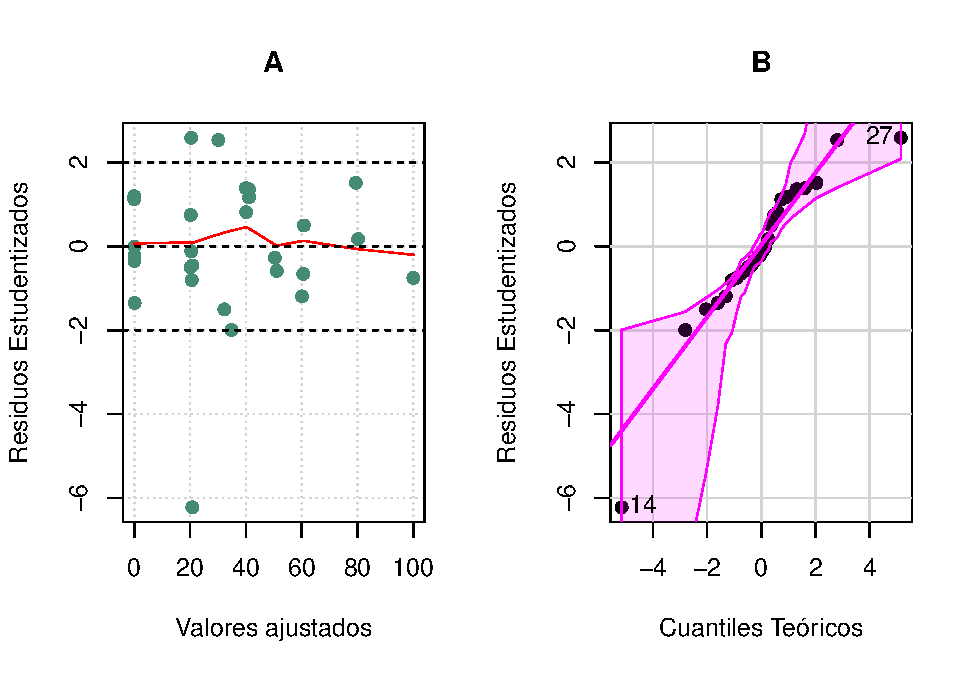
\includegraphics{Taller-2-Regresion-Multiple-Aplicada_files/figure-latex/unnamed-chunk-4-1.pdf}
{[}1{]} ``Shapiro Test''

\begin{verbatim}
Shapiro-Wilk normality test
\end{verbatim}

data: studres(model) W = 0.86458, p-value = 0.001868

{[}1{]} ``Breusch Pagan Test''

\begin{verbatim}
studentized Breusch-Pagan test
\end{verbatim}

data: model BP = 27.288, df = 24, p-value = 0.2912

Como no se cumple el supuesto de normalidad se procede a corregir
mediante el metodo de BoxCox y se verifica el cumplimiento de los
mismos.

\begin{Shaded}
\begin{Highlighting}[]
\NormalTok{model }\OtherTok{\textless{}{-}} \FunctionTok{lm}\NormalTok{(density}\FloatTok{+0.0000001} \SpecialCharTok{\textasciitilde{}}\NormalTok{ .}\SpecialCharTok{{-}}\NormalTok{NIR1}\SpecialCharTok{{-}}\NormalTok{NIR8}\SpecialCharTok{{-}}\NormalTok{NIR9}\SpecialCharTok{{-}}\NormalTok{NIR10}\SpecialCharTok{{-}}\NormalTok{NIR11}\SpecialCharTok{{-}}\NormalTok{NIR7, }\AttributeTok{data=}\NormalTok{X)}
\FunctionTok{lambda}\NormalTok{(model,}\SpecialCharTok{{-}}\DecValTok{3}\NormalTok{,}\DecValTok{3}\NormalTok{)}
\end{Highlighting}
\end{Shaded}

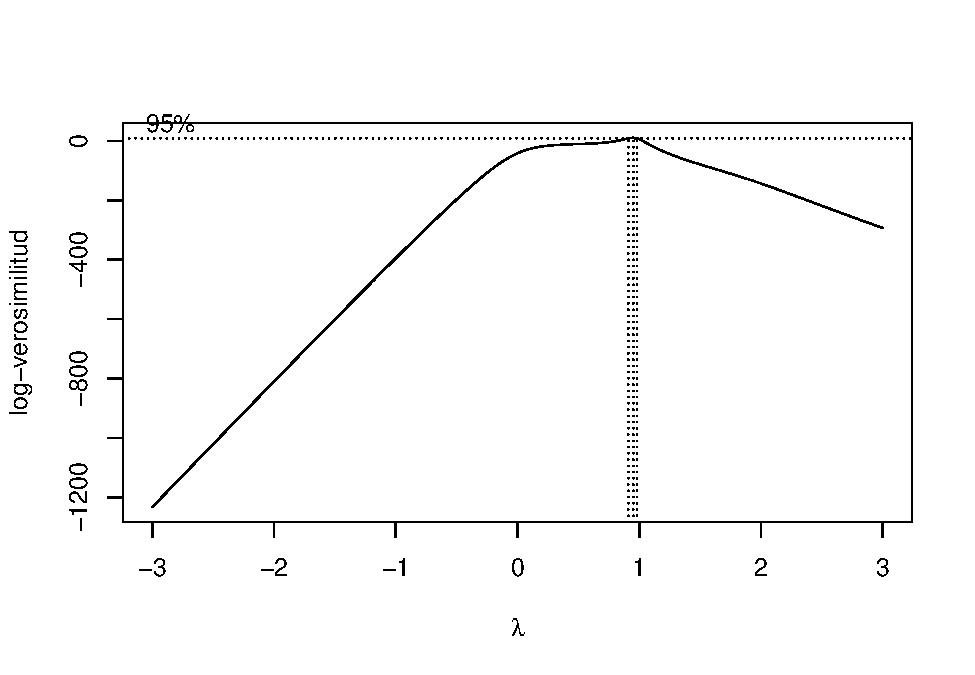
\includegraphics{Taller-2-Regresion-Multiple-Aplicada_files/figure-latex/unnamed-chunk-5-1.pdf}
{[}1{]} 0.95

\begin{Shaded}
\begin{Highlighting}[]
\NormalTok{model.box }\OtherTok{\textless{}{-}} \FunctionTok{lm}\NormalTok{(}\FunctionTok{I}\NormalTok{(density}\SpecialCharTok{\^{}}\FloatTok{0.96}\NormalTok{) }\SpecialCharTok{\textasciitilde{}}\NormalTok{.}\SpecialCharTok{{-}}\NormalTok{NIR1}\SpecialCharTok{{-}}\NormalTok{NIR8}\SpecialCharTok{{-}}\NormalTok{NIR9}\SpecialCharTok{{-}}\NormalTok{NIR10}\SpecialCharTok{{-}}\NormalTok{NIR11}\SpecialCharTok{{-}}\NormalTok{NIR7,}\AttributeTok{data=}\NormalTok{X)}
\FunctionTok{validaciongrafica}\NormalTok{(model.box)}
\end{Highlighting}
\end{Shaded}

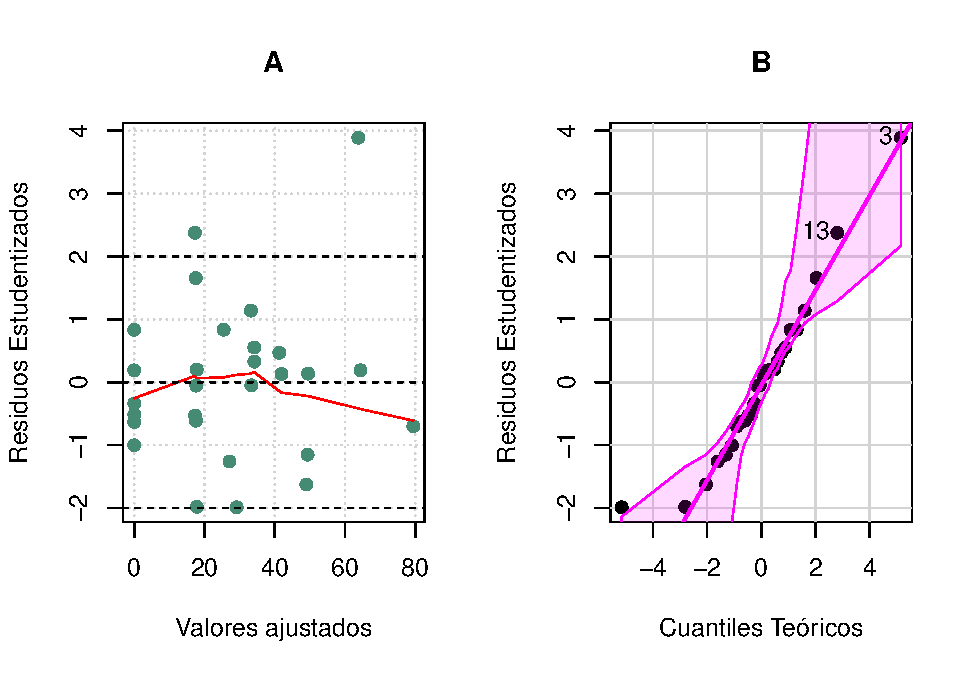
\includegraphics{Taller-2-Regresion-Multiple-Aplicada_files/figure-latex/unnamed-chunk-5-2.pdf}
{[}1{]} ``Shapiro Test''

\begin{verbatim}
Shapiro-Wilk normality test
\end{verbatim}

data: studres(model) W = 0.97774, p-value = 0.7934

{[}1{]} ``Breusch Pagan Test''

\begin{verbatim}
studentized Breusch-Pagan test
\end{verbatim}

data: model BP = 23.94, df = 24, p-value = 0.4651

Ya con los requerimentos necesarios para realizar regresión de LASSO, se
procede a calcular las estimaciones para distintos valores de
\(\lambda\) que se muestran en la siguiente figura:

\begin{Shaded}
\begin{Highlighting}[]
\NormalTok{X.}\OtherTok{\textless{}{-}}\FunctionTok{model.matrix}\NormalTok{(model.box)[,}\SpecialCharTok{{-}}\DecValTok{1}\NormalTok{]}
\NormalTok{lasso.mod }\OtherTok{\textless{}{-}} \FunctionTok{glmnet}\NormalTok{(X., X}\SpecialCharTok{$}\NormalTok{density, }\AttributeTok{alpha =} \DecValTok{1}\NormalTok{,}\AttributeTok{nlambda =} \DecValTok{100}\NormalTok{)}
\FunctionTok{plot}\NormalTok{(lasso.mod,}\AttributeTok{xvar=}\StringTok{\textquotesingle{}lambda\textquotesingle{}}\NormalTok{,}\AttributeTok{label=}\NormalTok{T,}\AttributeTok{lwd=}\DecValTok{2}\NormalTok{,}\AttributeTok{ylab=}\StringTok{\textquotesingle{}coeficientes de regresión\textquotesingle{}}\NormalTok{)}
\FunctionTok{abline}\NormalTok{(}\AttributeTok{h=}\DecValTok{0}\NormalTok{,}\AttributeTok{lty=}\DecValTok{2}\NormalTok{)}
\end{Highlighting}
\end{Shaded}

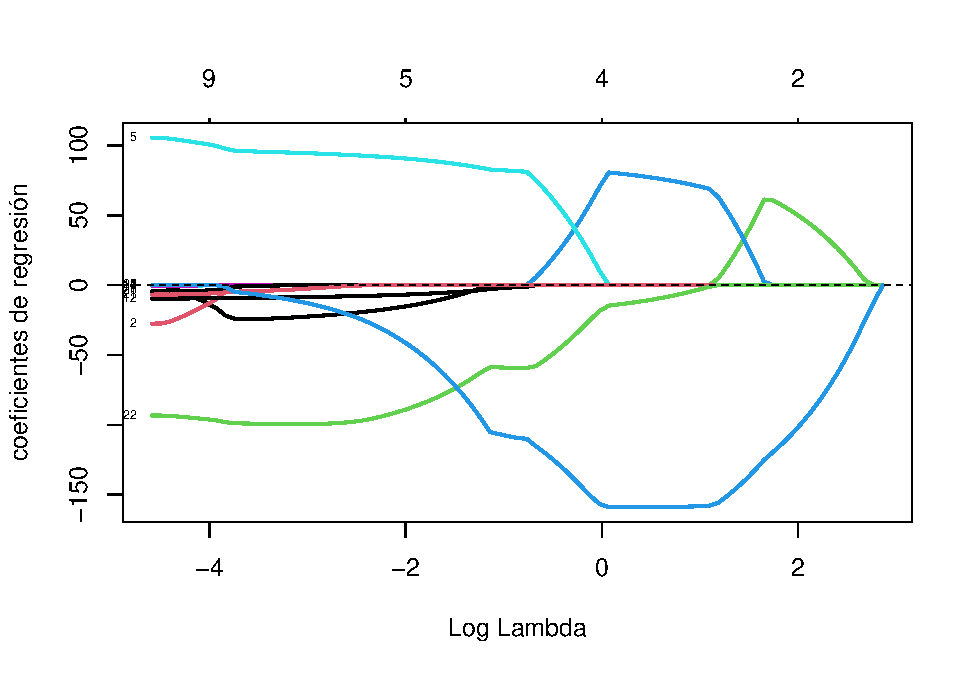
\includegraphics{Taller-2-Regresion-Multiple-Aplicada_files/figure-latex/unnamed-chunk-6-1.pdf}

Para identificar el valor de \(\lambda\) optimo se procede a realizar
validación cruzada.

\hypertarget{validaciuxf3n-cruzada}{%
\subsubsection{Validación cruzada}\label{validaciuxf3n-cruzada}}

Es un método para evaluar que tan bueno es un modelo para predecir
observaciones futuras de la población objeto de estudio. La muestra se
divide en dos grupos:

\begin{itemize}
\item
  Entrenamiento: Se usa para ajustar el modelo.
\item
  Validación: Se utiliza para validar el modelo ajustado.
\end{itemize}

\begin{Shaded}
\begin{Highlighting}[]
\NormalTok{lasso.cv }\OtherTok{\textless{}{-}}\FunctionTok{cv.glmnet}\NormalTok{(X., X}\SpecialCharTok{$}\NormalTok{density, }\AttributeTok{nfolds =} \DecValTok{4}\NormalTok{, }\AttributeTok{alpha =} \DecValTok{1}\NormalTok{,}\AttributeTok{nlambda =} \DecValTok{100}\NormalTok{)}
\FunctionTok{plot}\NormalTok{(lasso.cv)}
\end{Highlighting}
\end{Shaded}

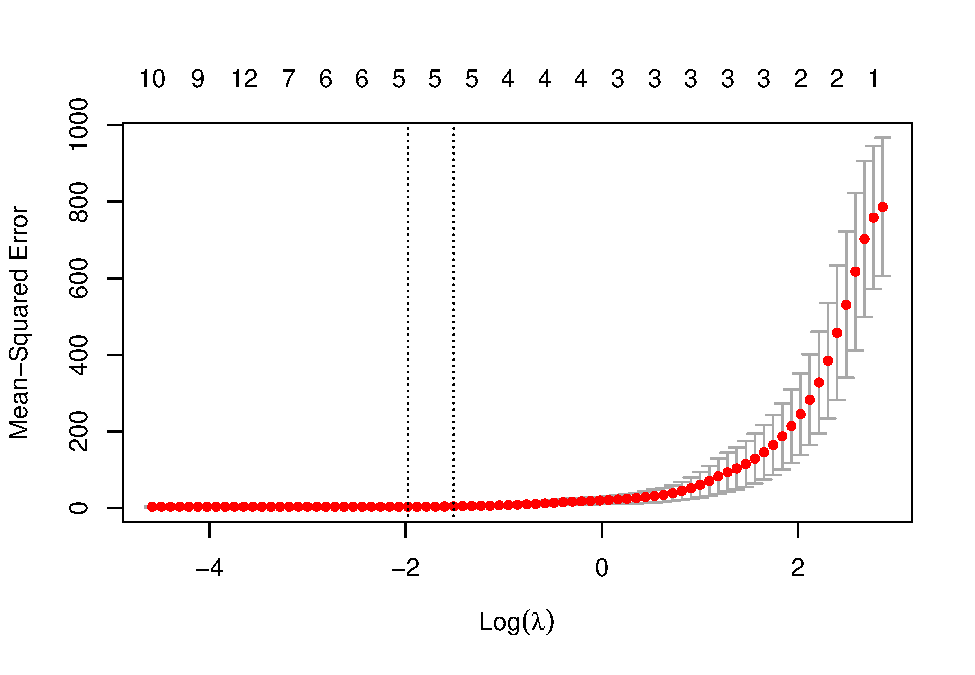
\includegraphics{Taller-2-Regresion-Multiple-Aplicada_files/figure-latex/unnamed-chunk-7-1.pdf}

\begin{Shaded}
\begin{Highlighting}[]
\NormalTok{est }\OtherTok{=} \FunctionTok{glmnet}\NormalTok{(X., X}\SpecialCharTok{$}\NormalTok{density, }\AttributeTok{alpha =} \DecValTok{1}\NormalTok{,}\AttributeTok{lambda =}\NormalTok{ lasso.cv}\SpecialCharTok{$}\NormalTok{lambda}\FloatTok{.1}\NormalTok{se)}
\NormalTok{est}\SpecialCharTok{$}\NormalTok{beta}
\end{Highlighting}
\end{Shaded}

24 x 1 sparse Matrix of class ``dgCMatrix'' s0 NIR2 -9.925178 NIR3 .\\
NIR4 .\\
NIR5 .\\
NIR6 87.822803 NIR12 .\\
NIR13 .\\
NIR14 .\\
NIR15 .\\
NIR16 .\\
NIR17 .\\
NIR18 -5.289614 NIR19 .\\
NIR20 .\\
NIR21 .\\
NIR22 .\\
NIR23 .\\
NIR24 .\\
NIR25 .\\
NIR26 .\\
NIR27 .\\
NIR28 -91.135757 NIR29 -43.247958 NIR30 .

\hypertarget{modelo-de-regresiuxf3n-multiple}{%
\section{Modelo de regresión
multiple}\label{modelo-de-regresiuxf3n-multiple}}

Con base en el proceso de selección de variables se ajusta el siguiente
modelo y se realiza la respectiva validación de supuestos:

\begin{Shaded}
\begin{Highlighting}[]
\NormalTok{model.lasso1}\OtherTok{\textless{}{-}} \FunctionTok{lm}\NormalTok{(density}\SpecialCharTok{\textasciitilde{}}\NormalTok{NIR2}\SpecialCharTok{+}\NormalTok{NIR6}\SpecialCharTok{+}\NormalTok{NIR18}\SpecialCharTok{+}\NormalTok{NIR28,}\AttributeTok{data=}\NormalTok{X)}
\FunctionTok{summary}\NormalTok{(model.lasso1)}
\end{Highlighting}
\end{Shaded}

Call: lm(formula = density \textasciitilde{} NIR2 + NIR6 + NIR18 +
NIR28, data = X)

Residuals: Min 1Q Median 3Q Max -2.1312 -0.9776 0.1102 0.8381 2.0416

Coefficients: Estimate Std. Error t value
Pr(\textgreater\textbar t\textbar)\\
(Intercept) 29.389 10.712 2.744 0.0116 *\\
NIR2 -26.257 3.892 -6.747 6.99e-07 \textbf{\emph{ NIR6 96.140 1.741
55.211 \textless{} 2e-16 }} NIR18 -9.055 1.905 -4.753 8.62e-05
\textbf{\emph{ NIR28 -109.939 5.818 -18.896 1.66e-15 }} --- Signif.
codes: 0 `\emph{\textbf{' 0.001 '}' 0.01 '}' 0.05 `.' 0.1 ' ' 1

Residual standard error: 1.169 on 23 degrees of freedom Multiple
R-squared: 0.9984, Adjusted R-squared: 0.9981 F-statistic: 3584 on 4 and
23 DF, p-value: \textless{} 2.2e-16

\begin{Shaded}
\begin{Highlighting}[]
\FunctionTok{validaciongrafica}\NormalTok{(model.lasso1)}
\end{Highlighting}
\end{Shaded}

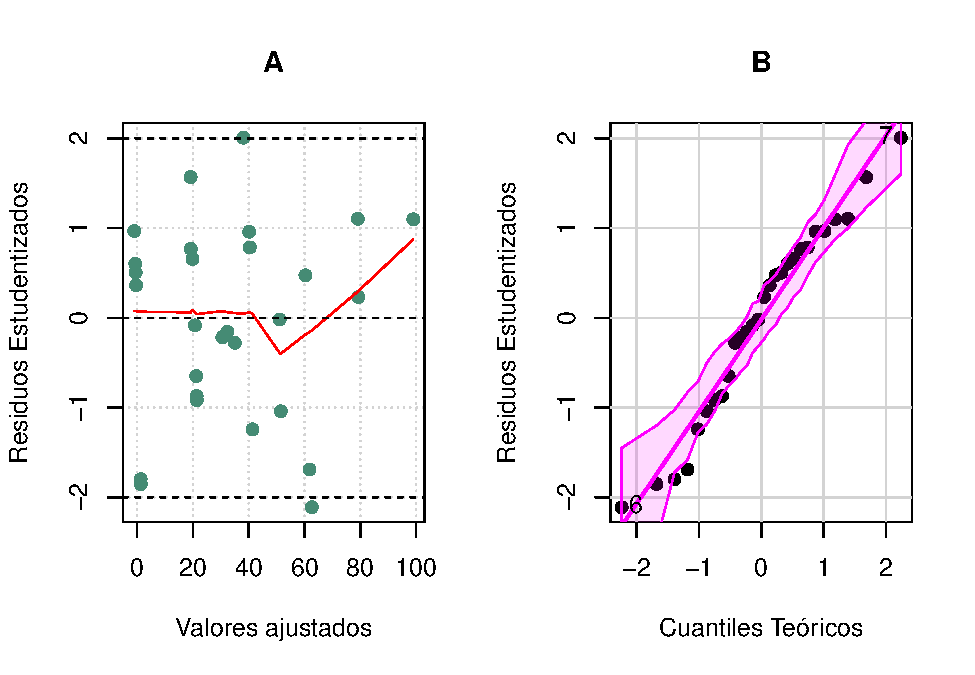
\includegraphics{Taller-2-Regresion-Multiple-Aplicada_files/figure-latex/unnamed-chunk-8-1.pdf}
{[}1{]} ``Shapiro Test''

\begin{verbatim}
Shapiro-Wilk normality test
\end{verbatim}

data: studres(model) W = 0.96468, p-value = 0.4471

{[}1{]} ``Breusch Pagan Test''

\begin{verbatim}
studentized Breusch-Pagan test
\end{verbatim}

data: model BP = 1.6317, df = 4, p-value = 0.8031

\hypertarget{section}{%
\subsection{}\label{section}}

\end{document}
